\subsection{Απάντηση Υποερωτήματος (β)}
\label{ssec:Solution_1.2}
\doublespacing

\par Η μηχανή μας δέχεται ουσιαστικά δέχεται ακριβώς δύο τιμές του δυαδικού συστήματος αρίθμησης, ίσου μήκους
μεταξύ τους και συμπεριλαμβανομένης της κενής λέξης (και άρα καμία τιμής).\\
Οι εγγραφές της ταινίας αρχίζουν και τελειώνουν υποχρεωτικά με κενό καθώς και οι δύο λέξεις διαχωρίζονται με κενό
ανάμεσα τους.\\
Άρα από τα δύο πρώτα ήδη καταλαβαίνουμε ότι αν οι λέξεις μας είναι κενές τότε έχουμε απλά τρία συνεχόμενα κενά στην
ταινία. Αυτό με τη σειρά του σημαίνει ότι έχουμε ουσιαστικά άπειρα κενά δεδομένου ότι η ταινία του θεωρητικού
μοντέλου είναι απείρου μήκους και κάθε θέση δεξιότερα του δεξιότερου (πλην κενού) συμβόλου, αποτελείτε από κενές
θέσεις.\\
Σε αυτή τη περίπτωση ουσιαστικά η έξοδος της μηχανής ισούται ακριβώς με την είσοδο (τρία κενά δίδονται, τρία κενά
λαμβάνονται).\\
Η άλλη περίπτωση είναι οι λέξεις αυτές να έχουν μη μηδενικό μήκος.\\
Στην περίπτωση αυτή η μηχανή θα αντικαταστήσει την αριστερή λέξη με το αποτέλεσμα της λογικής πράξης NAND μεταξύ
των δύο δυαδικών τιμών και την δεξιότερη με το αποτέλεσμα της λογικής πράξης AND μεταξύ τους.

\par
Εφόσον μπορούμε να λάβουμε κενές τιμές τότε βέλτιστο θα ήταν να τις ελέγξουμε εξ αρχής και άρα το πρώτο βήμα που
επιλέγουμε θα είναι ο έλεγχος για κενή πρώτη συμβολοσειρά.\\
Εφόσον όπως είπαμε ήδη οι δύο τιμές θα πρέπει να είναι ίσου μήκους, εάν η πρώτη μας συμβολοσειρά δεν περιέχει
κανένα σύμβολο τότε δεν θα περιέχει ούτε η δεύτερη.\\
Αυτό σημαίνει ότι απλά με μία κίνηση κεφαλής δεξιά και ανάγνωση μπορούμε ήδη να γνωρίζουμε αν η ταινία αποτελείτε
μόνο από κενές θέσεις ή όχι και να δρομολογήσουμε ανάλογα.

\par
Έπειτα παρατηρούμε ότι θα πρέπει να εκτελέσουμε τις λογικές πράξεις AND και NAND και να προβούμε σε αντικατάσταση
των αρχικών τιμών με τα αντίστοιχα αποτελέσματα αυτών των πράξεων.\\
Παρατηρούμε ότι για να εκτελέσουμε τη NAND ουσιαστικά εκτελούμε μία AND και κατόπιν παίρνουμε την άρνηση της, όντως
μία πιο περίπλοκη διαδικασία η μία της άλλης.\\
Άρα βάση αυτού αποφασίζομαι ότι θα ήταν βέλτιστο να υπολογίσουμε μόνο την AND και κατόπιν για την τιμή αποτέλεσμα
της NAND απλά να πάρουμε την άρνηση του προηγούμενου αποτελέσματος, κάνοντας έτσι ουσιαστικά δύο λογικές πράξεις
αντί για τρεις, συνολικά και για τις δύο τιμές μαζί.\\
Ουσιαστικά οι δύο διαδικασίες έχουν κοινό (αρχικό) μέρος και αντί να κατασκευάσουμε και να εκτελέσουμε δύο φορές
τον ίδιο αλγόριθμο, το κάνουμε μία φορά, με έναν υπολογισμό και για τα δύο και απλά προσθέτουμε τον επιπρόσθετο
υπολογισμό στο NAND τμήμα.\\
Τέλος με το πέρας των υπολογισμών και των μετατροπών, η κεφαλή θα πρέπει να μεταφέρεται ξανά πίσω στο πρώτο κενό
(όπου και βρίσκεται κατά την εκκίνηση).

\par
Τώρα παρατηρούμε ότι είναι πιθανότατο να έχουμε πρόβλημα με την απομνημόνευση του πια σύμβολα έχουν
αναγνωσθεί/υπολογισθεί, πια έχουν αντικατασταθεί και πια ακόμη περιμένουν τη σειρά τους. Με λίγα λόγια θα πρέπει να
βρούμε τρόπο ο αλγόριθμος να θυμάται τί έχει περάσει ή πειράξει.\\
Έχουμε σκεφθεί δύο μεθόδους, αλλά όπως πάντα είναι σχεδόν βέβαιο ότι υπάρχουν παραπάνω και επίσης δεν σημαίνει ότι
αυτές που δίδουμε είναι απαραίτητα οι πλέον αποδοτικές. Παρόλα αυτά πιστεύουμε ότι είναι επαρκώς αποδοτικές και
κατανοητές και δεν θα αφιερώσουμε παραπάνω χρόνο στην εύρεση κάτι καλύτερου που δεν γνωρίζουμε κατά πόσο υπάρχει
και με αμφίβολο το αν αξίζει τον επιπλέον κόπο.\\
Η πρώτη μέθοδος που δεν θα ακολουθηθεί τελικά, είναι να γράψουμε τα αποτελέσματα μετά το τρίτο εν σειρά κενό της
ταινίας (δηλαδή πέρα της όλης αρχικής εισόδου που απαιτεί η μηχανή) και κατόπιν να τα μεταφέρουμε (ταυτόχρονα
αντικαθιστώντας το σύμβολο στην θέση τους με κενό χαρακτήρα) επικαλύπτοντας τις αρχικές τιμές (σκεφτείτε το σαν
cut-paste). Με αυτόν τον τρόπο απαλλασσόμαστε μέρους της ανάγκης εισαγωγής πολλών επιπλέον προσωρινών συμβόλων που
θα εκτελούσαν χρέη δεικτών ώστε να γνωρίζουμε μέχρι που και τί έχουμε κάνει.\\
Η μέθοδος αυτή δεν θα προτιμηθεί διότι εάν μία τέτοια διαδικασία υλοποιηθεί, θα απαιτήσει πολλές παραπάνω και
μεγαλύτερες μετακινήσεις της κεφαλή, προκαλώντας έτσι μεγαλύτερες καθυστερήσεις στην παραλαβή της εξόδου και
αυξημένες φθορές στον όλο μηχανισμό (καθώς και επιπλέων καταναλώσεις ενέργειας κοκ). Το ερώτημα δεν μας ζητά να
λάβουμε κάτι τέτοιο υπόψιν και γνωρίζουμε ότι όσο αφορά τις ασκήσεις αυτές μιλάμε ξεκάθαρα για θεωρητικά μοντέλα
και μόνο, παρόλα αυτά θεωρούμε ότι είναι ορθό να σκεφτόμαστε με αυτόν τον τρόπο γενικότερα. Με λίγα λόγια στην δική
μας επίλυση, έμφαση θα δοθεί στην οικονομία κινήσεων της κεφαλής, επιπροσθέτως της ορθής επίλυσης.\\
Η δεύτερη λοιπόν μέθοδος και αυτή που τελικά θα επιλεχθεί, απαιτεί την χρήση παραπάνω χαρακτήρων των ελάχιστων που
απαιτούνται. Αυτοί οι παραπάνω χαρακτήρες θα είναι τουλάχιστον δύο καινούργια σύμβολα, το $T$ και το $F$, το πρώτο
από το True που θα αντικαθιστά τα 1 και το άλλο από το False που θα αντικαθιστά τα 0. Με αυτό το τρόπο πετυχαίνουμε
δύο πράγματα ταυτόχρονα: με ένα και μόνο σύμβολο γνωρίζει η μηχανή και τί έχει αντικατασταθεί ήδη με το αποτέλεσμα
της NAND ή AND και ταυτόχρονα τί τιμή έχει. Ενδεχομένως να χρειαστεί και τρίτο σύμβολο κατά την ανάγνωση ώστε να
θυμάται το σύστημα μέχρι που έχει φτάσει αυτή (η ανάγνωση) όπου σε αυτή τη περίπτωση θα χρησιμοποιήσουμε το σύμβολο
$\$$.\\
Τέλος θα πούμε ότι όπως και στην προηγούμενη άσκηση, έτσι και σε αυτή θα κατασκευάσουμε ανεξάρτητες μηχανές Turing
όπου η κάθε μία θα αναλαμβάνει μέρος του έργου (διαίρει και βασίλευε) και κατόπιν θα τις συνενώνουμε σε μία
παίρνοντας το ζητούμενο.

\par Η μηχανή $M_{S}$ θέλουμε απλά να ελέγχει αν η ταινία είναι κενή (ελέγχοντας αν υπάρχει έστω ένας χαρακτήρας
στη λέξη $x$) και αν ναι να μετακινεί την κεφαλή στη πρώτη θέση μετά την αρχή της ταινίας, η οποία θέση θα πρέπει
απαραίτητα να είναι κενή. Αυτό το πετυχαίνει κάνοντας μία μετακίνηση δεξιά ώστε να βρεθεί η κεφαλή εκεί που
αναμένετε (υποχρεωτικά) το πρώτο σύμβολο της λέξης και κατόπιν ελέγχει εάν αυτό όντως ανήκει στα σύμβολα της λέξης
ή όχι (άρα κενό) και δρομολογεί ανάλογα στην αντίστοιχη επόμενη μηχανή. Τον λόγο για τον οποίο δεν ελέγχουμε και το
$y$ τον έχουμε ήδη αναφέρει και είναι ότι απλά, $x$ και $y$ έχουν ίδιο μήκος και άρα αν το ένα είναι κενό, θα είναι
και το άλλο.
\[\text{Έλεγχος κενής λέξης}\,:\, M_S\,:\quad
L\,\overset{\sqcup}{\longleftarrow}\overset{\lor}{{\text{\large\bfseries
			R}}}\overset{0}{\longrightarrow}\, M_{0LR}\]
\reducevspace\reducevspace\reducevspace\reducevspace\reducevspace\reducevspace\reducevspace\reducevspace\reducevspace
\reducevspace\reducevspace\reducevspace\reducevspace\reducevspace\reducevspace\reducevspace\reducevspace\reducevspace
\reducevspace\reducevspace\reducevspace\reducevspace\reducevspace\reducevspace\reducevspace\reducevspace\reducevspace
\reducevspace\reducevspace\reducevspace\reducevspace\reducevspace\reducevspace\reducevspace\reducevspace\reducevspace
\[\qquad\qquad\qquad\qquad\qquad\qquad\qquad\qquad\quad\;\;\overset{1}{\longrightarrow}\, M_{1LR}\]
\reducevspace\reducevspace\reducevspace\reducevspace\reducevspace\reducevspace\reducevspace\reducevspace\reducevspace
Δοκιμή:
\reducevspace\reducevspace\reducevspace\reducevspace\reducevspace\reducevspace\reducevspace\reducevspace\reducevspace
\begin{itemize}
	\itemsep0em
	\item $|x| = |y| = |z| = |w| = 0 \;\Rightarrow\;\triangleright\, \underline{\sqcup}\, \sqcup \sqcup
	\xrightarrow{R} \triangleright\, \sqcup\, \underline{\sqcup}\, \sqcup \xrightarrow{\sqcup}
	\triangleright\, \underline{\sqcup}\,  \sqcup\, \sqcup  \quad$
	\textcolor{green}{\ding{51}}

	\item{ $|x| = |y| = |z| = |w| = n, n \geq 1 \;\Rightarrow\;\triangleright\, \underline{\sqcup}\, x_1\,...\,y_n
	\sqcup\, y_1\,...\,y_n\, \sqcup \xrightarrow{R}\\ \triangleright\, \sqcup\, \underline{x_1}\,...\,x_n\,
	\sqcup\, y_1\,...\,y_n\, \sqcup \xrightarrow{0} M_{0LR} \quad$ \textcolor{green}{\ding{51}}\\
	\makebox[4.3cm]{\hfill}$\xrightarrow{1} M_{1LR} \quad$ \textcolor{green}{\ding{51}}}
\end{itemize}
\clearpage

\par Η $M_{0LR}$ διαβάζει, υπολογίζει και αντικαθιστά από αριστερά προς τα δεξιά για $x_n\,=\,0$.
\reducevspace\reducevspace\reducevspace\reducevspace\reducevspace\reducevspace\reducevspace\reducevspace\reducevspace
\reducevspace\reducevspace\reducevspace\reducevspace\reducevspace\reducevspace\reducevspace\reducevspace\reducevspace
%\[\text{Υπολογισμός/Αντικατάσταση Αριστερά προς Δεξιά}\,:\, M_{0LR}\,:\]
\[\overset{\lor}{{\text{\large\bfseries T}}}\,R_\sqcup\, \longrightarrow\,
\overset{F,\,T}{\overset{\botcircleleft}{R}}
\overset{0,\,1}{\longrightarrow}\,
F\,R\,\xrightarrow{0} M_{0RL}\]
\reducevspace\reducevspace\reducevspace\reducevspace\reducevspace\reducevspace\reducevspace
\reducevspace\reducevspace\reducevspace\reducevspace\reducevspace\reducevspace\reducevspace
\reducevspace\reducevspace\reducevspace\reducevspace\reducevspace\reducevspace\reducevspace
\reducevspace\reducevspace\reducevspace\reducevspace\reducevspace\reducevspace\reducevspace
\[\qquad\qquad\qquad\qquad\quad\;\;\;\,\xrightarrow{1}\, M_{1RL}\]

\reducevspace\reducevspace\reducevspace\reducevspace\reducevspace\reducevspace\reducevspace\reducevspace\reducevspace
\reducevspace\reducevspace\reducevspace\reducevspace\reducevspace\reducevspace\reducevspace\reducevspace\reducevspace
\reducevspace\reducevspace\reducevspace\reducevspace\reducevspace\reducevspace\reducevspace\reducevspace\reducevspace
\reducevspace\reducevspace\reducevspace\reducevspace\reducevspace\reducevspace\reducevspace\reducevspace\reducevspace
\[\qquad\qquad\qquad\qquad\quad\xrightarrow{\sqcup}\, M_T\]
\reducevspace\reducevspace\reducevspace\reducevspace\reducevspace\reducevspace\reducevspace\reducevspace\reducevspace
Δοκιμή:
\reducevspace\reducevspace\reducevspace\reducevspace\reducevspace\reducevspace\reducevspace\reducevspace\reducevspace
\begin{itemize}
	\itemsep0em
	\item $x\,=\,0,\; y\,=c,\; c\in\{0,\,1\} \;\xRightarrow{M_S}\;
	\triangleright\, \sqcup\, \underline{0}\, \sqcup\, c\, \sqcup\,\xrightarrow{TR_\sqcup}\;
	\triangleright\, \sqcup\, T\, \underline{\sqcup}\, c\, \sqcup\,
	\xrightarrow{\overset{F,\,T}{\overset{\botcircleleft}{R}}\xrightarrow{0,\,1}F}\;
	\triangleright\, \sqcup\, T\, \sqcup\, \underline{F}\, \sqcup\, \xrightarrow{R}\;
	\triangleright\, \sqcup\, T\, \sqcup\, F\, \underline{\sqcup}\, \xrightarrow{\sqcup} M_T
	\quad$ \textcolor{green}{\ding{51}}

	\item $x\,=\,0c,\; y\,=cd,\; c\in\{0,\,1\},\,d\in\{0,\,1\} \;\xRightarrow{M_S}\;
	\triangleright\, \sqcup\, \underline{0}\, c\, \sqcup\, c\, d\, \sqcup\,\xrightarrow{TR_\sqcup}\;$\\$
	\triangleright\, \sqcup\, T\, c\, \underline{\sqcup}\, c\, d\, \sqcup\,
	\xrightarrow{\overset{F,\,T}{\overset{\botcircleleft}{R}}\xrightarrow{0,\,1}F}\;
	\triangleright\, \sqcup\, T\, c\, \sqcup\, \underline{F}\, d\, \sqcup\, \xrightarrow{R}\;
	\triangleright\, \sqcup\, T\, c\, \sqcup\, F\, \underline{d}\, \sqcup\, \xrightarrow{0}\; M_{0RL}
	\quad$\textcolor{green}{\ding{51}}\\
	\makebox[11.32cm]{\hfill} $\xrightarrow{1}\; M_{1RL}\quad$\textcolor{green}{\ding{51}}
\end{itemize}


\par Η $M_{0RL}$ διαβάζει, υπολογίζει και αντικαθιστά από δεξιά προς τα αριστερά για $y_n\,=\,0$.
\reducevspace\reducevspace\reducevspace\reducevspace\reducevspace\reducevspace\reducevspace\reducevspace\reducevspace
\reducevspace\reducevspace\reducevspace\reducevspace\reducevspace\reducevspace\reducevspace\reducevspace\reducevspace
%\[\text{Υπολογισμός/Αντικατάσταση Δεξιά προς Αριστερά}\,:\, M_{0LR}\,:\]
\[\overset{\lor}{{\text{\large\bfseries F}}}\,L_\sqcup\, \longrightarrow\,
\overset{0,\,1}{\overset{\botcircleleft}{L}}
\overset{F,\,T}{\longrightarrow}\, R\,T\,R\,\xrightarrow{0} M_{0LR}\]
\reducevspace\reducevspace\reducevspace\reducevspace\reducevspace\reducevspace\reducevspace
\reducevspace\reducevspace\reducevspace\reducevspace\reducevspace\reducevspace\reducevspace
\reducevspace\reducevspace\reducevspace\reducevspace\reducevspace\reducevspace\reducevspace
\reducevspace\reducevspace\reducevspace\reducevspace\reducevspace\reducevspace\reducevspace
\[\qquad\qquad\qquad\qquad\qquad\;\;\,\xrightarrow{1}\, M_{1LR}\]

\reducevspace\reducevspace\reducevspace\reducevspace\reducevspace\reducevspace\reducevspace\reducevspace\reducevspace
\reducevspace\reducevspace\reducevspace\reducevspace\reducevspace\reducevspace\reducevspace\reducevspace\reducevspace
\reducevspace\reducevspace\reducevspace\reducevspace\reducevspace\reducevspace\reducevspace\reducevspace\reducevspace
\reducevspace\reducevspace\reducevspace\reducevspace\reducevspace\reducevspace\reducevspace\reducevspace\reducevspace
\[\qquad\qquad\qquad\qquad\qquad\qquad\;\;\xrightarrow{\sqcup}\, R_\sqcup \rightarrow M_T\]
\reducevspace\reducevspace\reducevspace\reducevspace\reducevspace\reducevspace\reducevspace\reducevspace\reducevspace
Δοκιμή:
\reducevspace\reducevspace\reducevspace\reducevspace\reducevspace\reducevspace\reducevspace\reducevspace\reducevspace
\begin{itemize}
	\itemsep0em
	\item $x\,=\,0c,\; y\,=00,\; c\in\{0,\,1\} \;\xRightarrow{M_S}\;
	\triangleright\, \sqcup\, T\, c\, \sqcup\, F\, \underline{0}\, \sqcup\; \xrightarrow{FL_\sqcup}\;
	\triangleright\, \sqcup\, T\, c\, \underline{\sqcup}\, F\, F\, \sqcup\;
	\xrightarrow{\overset{0,\,1}{\overset{\botcircleleft}{L}}\xrightarrow{F,\,T}R}\;
	\triangleright\, \sqcup\, T\, \underline{c}\, \sqcup\, F\, F\, \sqcup\; \xrightarrow{TR}\;
	\triangleright\, \sqcup\, T\, T\, \underline{\sqcup}\, F\, F\, \sqcup\;
	\xrightarrow{\xrightarrow{\sqcup}R_\sqcup}\;
	\triangleright\, \sqcup\, T\, T\, \sqcup\, F\, F\, \underline{\sqcup}\; \xrightarrow{\sqcup}\; M_T
	\quad$ \textcolor{green}{\ding{51}}
	\clearpage
	\item $x\,=\,0cd,\; y\,=00c,\; d\in \{0,\,1\},\; c\in\{0,\,1\},\,d\in\{0,\,1\} \;\xRightarrow{M_S}\\
	\triangleright\, \sqcup\, T\, c\, d\, \sqcup\, F\, \underline{0}\, c\, \sqcup\; \xrightarrow{FL_\sqcup}\;
	\triangleright\, \sqcup\, T\, c\, d\, \underline{\sqcup}\, F\, F\, c\, \sqcup\;
	\xrightarrow{\overset{0,\,1}{\overset{\botcircleleft}{L}}\xrightarrow{F,\,T}R}\;
	\triangleright\, \sqcup\, T\, \underline{c}\, d\, \sqcup\, F\, F\, c\, \sqcup\; \xrightarrow{TR}\;
	\triangleright\, \sqcup\, T\, T\, \underline{d}\, \sqcup\, F\, F\, c\, \sqcup\; \xrightarrow{0}\; M_{0LR}
	\quad$ \textcolor{green}{\ding{51}}\\
	\makebox[3.8cm]{\hfill}$\xrightarrow{1}\; M_{1LR} \quad$ \textcolor{green}{\ding{51}}
\end{itemize}

%%%%%%%%%%%%%%%%%%%%%%%%%%%%
% Here forth is for case "1"
%%%%%%%%%%%%%%%%%%%%%%%%%%%%%


\par Η $M_{1LR}$ διαβάζει, υπολογίζει και αντικαθιστά από αριστερά προς τα δεξιά για $x_n\,=\,1$.
\reducevspace\reducevspace\reducevspace\reducevspace\reducevspace\reducevspace\reducevspace\reducevspace\reducevspace
\reducevspace\reducevspace\reducevspace\reducevspace\reducevspace\reducevspace\reducevspace\reducevspace\reducevspace
%\[\text{Υπολογισμός/Αντικατάσταση Αριστερά προς Δεξιά}\,:\, M_{0LR}\,:\]
\[\overset{\lor}{{\text{\large\bfseries \$}}}\,R_\sqcup\, \longrightarrow\,
\overset{F,\,T}{\overset{\botcircleleft}{R}}\, \xrightarrow{0} F\, L_\$\, T\, R\, \xrightarrow{\sqcup}\, R_\sqcup\,
\rightarrow\, M_T \]
\reducevspace\reducevspace\reducevspace\reducevspace\reducevspace\reducevspace\reducevspace
\reducevspace\reducevspace\reducevspace\reducevspace\reducevspace\reducevspace\reducevspace
\reducevspace\reducevspace\reducevspace\reducevspace\reducevspace\reducevspace\reducevspace
\reducevspace\reducevspace\reducevspace\reducevspace\reducevspace\reducevspace\reducevspace
\[\qquad\qquad\qquad\qquad\qquad\qquad\qquad\quad\;\, \xrightarrow{0}\, M_{0LR}\]
\reducevspace\reducevspace\reducevspace\reducevspace\reducevspace\reducevspace\reducevspace
\reducevspace\reducevspace\reducevspace\reducevspace\reducevspace\reducevspace\reducevspace
\reducevspace\reducevspace\reducevspace\reducevspace\reducevspace\reducevspace\reducevspace
\reducevspace\reducevspace\reducevspace\reducevspace\reducevspace\reducevspace\reducevspace
\[\qquad\qquad\qquad\qquad\qquad\qquad\qquad\quad\;\, \xrightarrow{1}\, M_{1LR}\]

\reducevspace\reducevspace\reducevspace\reducevspace\reducevspace\reducevspace\reducevspace\reducevspace\reducevspace
\reducevspace\reducevspace\reducevspace\reducevspace\reducevspace\reducevspace\reducevspace\reducevspace\reducevspace
\reducevspace\reducevspace\reducevspace\reducevspace\reducevspace\reducevspace\reducevspace\reducevspace\reducevspace
\reducevspace\reducevspace\reducevspace\reducevspace\reducevspace\reducevspace\reducevspace\reducevspace\reducevspace
\[\qquad\qquad\qquad\, \xrightarrow{1} T\, L_\$\, F\, R\, \xrightarrow{\sqcup}\, R_\sqcup\, \rightarrow\, M_T
\]
\reducevspace\reducevspace\reducevspace\reducevspace\reducevspace\reducevspace\reducevspace
\reducevspace\reducevspace\reducevspace\reducevspace\reducevspace\reducevspace\reducevspace
\reducevspace\reducevspace\reducevspace\reducevspace\reducevspace\reducevspace\reducevspace
\reducevspace\reducevspace\reducevspace\reducevspace\reducevspace\reducevspace\reducevspace
\[\qquad\qquad\qquad\qquad\qquad\qquad\qquad\quad\;\, \xrightarrow{0}\, M_{0LR}\]
\reducevspace\reducevspace\reducevspace\reducevspace\reducevspace\reducevspace\reducevspace
\reducevspace\reducevspace\reducevspace\reducevspace\reducevspace\reducevspace\reducevspace
\reducevspace\reducevspace\reducevspace\reducevspace\reducevspace\reducevspace\reducevspace
\reducevspace\reducevspace\reducevspace\reducevspace\reducevspace\reducevspace\reducevspace
\[\qquad\qquad\qquad\qquad\qquad\qquad\qquad\quad\;\, \xrightarrow{1}\, M_{1LR}\]
\reducevspace\reducevspace\reducevspace\reducevspace\reducevspace\reducevspace\reducevspace\reducevspace\reducevspace
Δοκιμή:
\reducevspace\reducevspace\reducevspace\reducevspace\reducevspace\reducevspace\reducevspace\reducevspace\reducevspace
\begin{itemize}
	\itemsep0em
	\item $x\,=\,1,\; y\,=0 \;\xRightarrow{M_S}\;
	\triangleright\, \sqcup\, \underline{1}\, \sqcup\, 0\, \sqcup\,\xrightarrow{\$R_\sqcup}\;
	\triangleright\, \sqcup\, \$\, \underline{\sqcup}\, 0\, \sqcup\,
	\xrightarrow{\overset{F,\,T}{\overset{\botcircleleft}{R}}\xrightarrow{0}F}\;
	\triangleright\, \sqcup\, \$\, \sqcup\, \underline{F}\, \sqcup\, \xrightarrow{L_\$TR}\;
	\triangleright\, \sqcup\, T\, \underline{\sqcup}\, F\, \sqcup\, \;\xrightarrow{\xrightarrow{\sqcup}R_\sqcup}
	\triangleright\, \sqcup\, T\, \sqcup\, F\, \underline{\sqcup} \;\xrightarrow{\sqcup}\; M_T
	\quad$\textcolor{green}{\ding{51}}

	\item $x\,=\,1,\; y\,=1 \;\xRightarrow{M_S}\;
	\triangleright\, \sqcup\, \underline{1}\, \sqcup\, 1\, \sqcup\,\xrightarrow{\$R_\sqcup}\;
	\triangleright\, \sqcup\, \$\, \underline{\sqcup}\, 1\, \sqcup\,
	\xrightarrow{\overset{F,\,T}{\overset{\botcircleleft}{R}}\xrightarrow{1}F}\;
	\triangleright\, \sqcup\, \$\, \sqcup\, \underline{T}\, \sqcup\, \xrightarrow{L_\$TR}\;
	\triangleright\, \sqcup\, F\, \underline{\sqcup}\, T\, \sqcup\, \;\xrightarrow{\xrightarrow{\sqcup}R_\sqcup}
	\triangleright\, \sqcup\, F\, \sqcup\, T\, \underline{\sqcup} \;\xrightarrow{\sqcup}\; M_T
	\quad$\textcolor{green}{\ding{51}}

	\item $x\,=\,1c,\; y\,=0c,\; c\in\{0,\,1\} \;\xRightarrow{M_S}\;
	\triangleright\, \sqcup\, \underline{1}\, c\, \sqcup\, 0\, c\, \sqcup\,\xrightarrow{\$R_\sqcup}\;
	\triangleright\, \sqcup\, \$\, c\, \underline{\sqcup}\, 0\, c\, \sqcup\\
	\xrightarrow{\overset{F,\,T}{\overset{\botcircleleft}{R}}\xrightarrow{0}F}\;
	\triangleright\, \sqcup\, \$\, c\, \sqcup\, \underline{F}\, c\, \sqcup\, \xrightarrow{L_\$TR}\;
	\triangleright\, \sqcup\, T\, \underline{c}\, \sqcup\, F\, c\, \sqcup\,
	\;\xrightarrow{0} M_{OLR}
	\quad$\textcolor{green}{\ding{51}}
	\makebox[11.3cm]{\hfill} $\xrightarrow{1}\; M_{1LR}\quad\,$ \textcolor{green}{\ding{51}}
\end{itemize}
\clearpage

\par Η $M_{1RL}$ διαβάζει, υπολογίζει και αντικαθιστά από δεξιά προς τα αριστερά για $y_n\,=\,1$.
\reducevspace\reducevspace\reducevspace\reducevspace\reducevspace\reducevspace\reducevspace\reducevspace\reducevspace
\reducevspace\reducevspace\reducevspace\reducevspace\reducevspace\reducevspace\reducevspace\reducevspace\reducevspace
%\[\text{Υπολογισμός/Αντικατάσταση Δεξιά προς Αριστερά}\,:\, M_{0LR}\,:\]
\[\overset{\lor}{{\text{\large\bfseries \$}}}\,L_\sqcup\, \longrightarrow\,
\overset{0,\,1}{\overset{\botcircleleft}{L}}\, \xrightarrow{T,\,F}\,R\,\xrightarrow{0} T\, R_\$\, F\, R\,
\xrightarrow{\sqcup}\, M_T \]
\reducevspace\reducevspace\reducevspace\reducevspace\reducevspace\reducevspace\reducevspace
\reducevspace\reducevspace\reducevspace\reducevspace\reducevspace\reducevspace\reducevspace
\reducevspace\reducevspace\reducevspace\reducevspace\reducevspace\reducevspace\reducevspace
\reducevspace\reducevspace\reducevspace\reducevspace\reducevspace\reducevspace\reducevspace
\[\qquad\qquad\qquad\qquad\qquad\qquad\qquad\quad\;\, \xrightarrow{0}\, M_{0LR}\]
\reducevspace\reducevspace\reducevspace\reducevspace\reducevspace\reducevspace\reducevspace
\reducevspace\reducevspace\reducevspace\reducevspace\reducevspace\reducevspace\reducevspace
\reducevspace\reducevspace\reducevspace\reducevspace\reducevspace\reducevspace\reducevspace
\reducevspace\reducevspace\reducevspace\reducevspace\reducevspace\reducevspace\reducevspace
\[\qquad\qquad\qquad\qquad\qquad\qquad\qquad\quad\;\, \xrightarrow{1}\, M_{1LR}\]

\reducevspace\reducevspace\reducevspace\reducevspace\reducevspace\reducevspace\reducevspace\reducevspace\reducevspace
\reducevspace\reducevspace\reducevspace\reducevspace\reducevspace\reducevspace\reducevspace\reducevspace\reducevspace
\reducevspace\reducevspace\reducevspace\reducevspace\reducevspace\reducevspace\reducevspace\reducevspace\reducevspace
\reducevspace\reducevspace\reducevspace\reducevspace\reducevspace\reducevspace\reducevspace\reducevspace\reducevspace
\[\qquad\qquad\qquad\qquad\quad\, \xrightarrow{1} F\, R_\$\, T\, R\, \xrightarrow{\sqcup}\, M_T
\]
\reducevspace\reducevspace\reducevspace\reducevspace\reducevspace\reducevspace\reducevspace
\reducevspace\reducevspace\reducevspace\reducevspace\reducevspace\reducevspace\reducevspace
\reducevspace\reducevspace\reducevspace\reducevspace\reducevspace\reducevspace\reducevspace
\reducevspace\reducevspace\reducevspace\reducevspace\reducevspace\reducevspace\reducevspace
\[\qquad\qquad\qquad\qquad\qquad\qquad\qquad\quad\;\, \xrightarrow{0}\, M_{0LR}\]
\reducevspace\reducevspace\reducevspace\reducevspace\reducevspace\reducevspace\reducevspace
\reducevspace\reducevspace\reducevspace\reducevspace\reducevspace\reducevspace\reducevspace
\reducevspace\reducevspace\reducevspace\reducevspace\reducevspace\reducevspace\reducevspace
\reducevspace\reducevspace\reducevspace\reducevspace\reducevspace\reducevspace\reducevspace
\[\qquad\qquad\qquad\qquad\qquad\qquad\qquad\quad\;\, \xrightarrow{1}\, M_{1LR}\]
\reducevspace\reducevspace\reducevspace\reducevspace\reducevspace\reducevspace\reducevspace
\reducevspace\reducevspace\reducevspace\reducevspace\reducevspace\reducevspace\reducevspace
\reducevspace\reducevspace\reducevspace\reducevspace\reducevspace\reducevspace\reducevspace
Δοκιμή:
\reducevspace\reducevspace\reducevspace\reducevspace\reducevspace\reducevspace\reducevspace\reducevspace\reducevspace
\begin{itemize}
	\itemsep0em
	\item $x\,=\,00,\; y\,=01 \;\xRightarrow{M_{0LR}}\;
	\triangleright\, \sqcup\, T\, 0\, \sqcup\, F\, \underline{1}\, \sqcup\; \xrightarrow{\$L_\sqcup}\;
	\triangleright\, \sqcup\, T\, 0\, \underline{\sqcup}\, F\, \$\, \sqcup\;
	\xrightarrow{\overset{0,\,1}{\overset{\botcircleleft}{L}}\xrightarrow{F,\,T}R}\;
	\triangleright\, \sqcup\, T\, \underline{0}\, \sqcup\, F\, \$\, \sqcup\; \xrightarrow{\xrightarrow{0}TR_\$FR}\;
	\triangleright\, \sqcup\, T\, T\, \sqcup\, F\, F\, \underline{\sqcup}\;\xrightarrow{\sqcup}\; M_T
	\quad$ \textcolor{green}{\ding{51}}

	\item $x\,=\,01,\; y\,=01 \;\xRightarrow{M_{0LR}}\;
	\triangleright\, \sqcup\, T\, 1\, \sqcup\, F\, \underline{1}\, \sqcup\; \xrightarrow{\$L_\sqcup}\;
	\triangleright\, \sqcup\, T\, 1\, \underline{\sqcup}\, F\, \$\, \sqcup\;
	\xrightarrow{\overset{0,\,1}{\overset{\botcircleleft}{L}}\xrightarrow{F,\,T}R}\;
	\triangleright\, \sqcup\, T\, \underline{1}\, \sqcup\, F\, \$\, \sqcup\; \xrightarrow{\xrightarrow{1}TR_\$FR}\;
	\triangleright\, \sqcup\, T\, F\, \sqcup\, F\, T\, \underline{\sqcup}\;\xrightarrow{\sqcup}\; M_T
	\quad$ \textcolor{green}{\ding{51}}

	\item $x\,=\,00c,\; y\,=01c,\; c\in\{0,\,1\} \;\xRightarrow{M_{0LR}}\;
	\triangleright\, \sqcup\, T\, 0\, c\, \sqcup\, F\, \underline{1}\, c\, \sqcup\; \xrightarrow{FL_\sqcup}\;
	\\ \triangleright\, \sqcup\, T\, 0\, c\, \underline{\sqcup}\, F\, \$\, c\, \sqcup\;
	\xrightarrow{\overset{0,\,1}{\overset{\botcircleleft}{L}}\xrightarrow{F,\,T}R}\;
	\triangleright\, \sqcup\, T\, \underline{0}\, c\, \sqcup\, F\, \$\, c\, \sqcup\;
	\xrightarrow{\xrightarrow{0}TR_\$FR}\;\\
	\triangleright\, \sqcup\, T\, T\, c\, \sqcup\, F\, F\, \underline{c}\, \sqcup\; \xrightarrow{0}\; M_{0RL}
	\quad$ \textcolor{green}{\ding{51}}\\
	\makebox[3.7cm]{\hfill}$\xrightarrow{1}\; M_{1RL} \quad$ \textcolor{green}{\ding{51}}
\end{itemize}

%\clearpage
\par H $M_T$ ενεργοποιείτε όταν οι δύο λέξεις ($z,\,w$) έχουν υπολογισθεί και κάνει τη μετάφραση από συμβολισμό
$F,\,T$ σε $0,\,1$. Ταυτόχρονα ο τρόπους που μετακινείτε στη ταινία για να κάνει την μετάφραση, του επιτρέπει
ταυτόχρονα να τερματίσει τη διαδικασία κατά την ολοκλήρωση της, με την κεφαλή στην αναμενόμενη από τις απαιτήσεις
θέση.

\reducevspace\reducevspace\reducevspace\reducevspace\reducevspace\reducevspace\reducevspace
\[\overset{\lor}{{\text{\large\bfseries L}}} \;\xrightarrow{F}\; 0 \rightarrow M_T \]
\reducevspace\reducevspace\reducevspace\reducevspace\reducevspace\reducevspace\reducevspace
\reducevspace\reducevspace\reducevspace\reducevspace\reducevspace\reducevspace\reducevspace
\reducevspace\reducevspace\reducevspace\reducevspace\reducevspace\reducevspace\reducevspace
\reducevspace\reducevspace\reducevspace\reducevspace\reducevspace\reducevspace\reducevspace
\[\quad\; \;\xrightarrow{T}\; 1 \rightarrow M_T\]
\reducevspace\reducevspace\reducevspace\reducevspace\reducevspace\reducevspace\reducevspace
\reducevspace\reducevspace\reducevspace\reducevspace\reducevspace\reducevspace\reducevspace
\reducevspace\reducevspace\reducevspace\reducevspace\reducevspace\reducevspace\reducevspace
\reducevspace\reducevspace\reducevspace\reducevspace\reducevspace\reducevspace\reducevspace
\[\xrightarrow{\sqcup}\; M_T \;\;\]
\reducevspace\reducevspace\reducevspace\reducevspace\reducevspace\reducevspace\reducevspace
\reducevspace\reducevspace\reducevspace\reducevspace\reducevspace\reducevspace\reducevspace
\reducevspace\reducevspace\reducevspace\reducevspace\reducevspace\reducevspace\reducevspace
\reducevspace\reducevspace\reducevspace\reducevspace\reducevspace\reducevspace\reducevspace
\[\xrightarrow{\triangleright}\; R \quad\]
\reducevspace\reducevspace\reducevspace\reducevspace\reducevspace\reducevspace\reducevspace
\reducevspace\reducevspace\reducevspace\reducevspace\reducevspace\reducevspace\reducevspace
Δοκιμή:
\reducevspace\reducevspace\reducevspace\reducevspace\reducevspace\reducevspace\reducevspace\reducevspace\reducevspace
\begin{itemize}
	\itemsep0em
	\item $x = 11,\, y = 01,\, \;\Rightarrow\;
	\triangleright\, \sqcup\, T\, F\, \sqcup\, F\,T\, \underline{\sqcup} \;\xrightarrow{L}\;
	\triangleright\, \sqcup\, T\, F\, \sqcup\, F\, \underline{T}\, \sqcup \;\xrightarrow{\xrightarrow{T}1}\;
	\triangleright\, \sqcup\, T\, F\, \sqcup\, F\, \underline{1}\, \sqcup
	\;\xrightarrow{M_T\rightarrow L\xrightarrow{F}0}\;
	\triangleright\, \sqcup\, T\, F\, \sqcup\, \underline{0}\, 1\, \sqcup
	\;\xrightarrow{M_T\rightarrow L\xrightarrow{\sqcup}M_T\rightarrow L\xrightarrow{F}0}\;
	\triangleright\, \sqcup\, T\, \underline{0}\, \sqcup\, 0\, 1\, \sqcup
	\;\xrightarrow{M_T\rightarrow L\xrightarrow{T}1}\;
	\triangleright\, \sqcup\, \underline{1}\, 0\, \sqcup\, 0\, 1\, \sqcup
	\;\xrightarrow{M_T\rightarrow L\xrightarrow{\sqcup}M_T\rightarrow L\xrightarrow{\triangleright} R}\;
	\triangleright\, \underline{\sqcup}\, 1\, 0\, \sqcup\, 0\, 1\, \sqcup
	\quad$ \textcolor{green}{\ding{51}}
\end{itemize}

\par Σχεδιάζουμε γραφικά τη διασύνδεση των μηχανών μεταξύ τους και κατόπιν επανασχεδιάζουμε αντικαθιστώντας τες με
την αντίστοιχη εσωτερική λειτουργία τους, έτσι ώστε να καταλήξουμε στο ζητούμενο.
Κάναμε τροποποιήσεις ώστε να συγχωνευτούν κάποιες διαδικασίες. Για παράδειγμα σε περίπτωση κενής
εισόδου, η $M_S$ μεταβαίνει στην $M_T$, μεταβιβάζοντας την ευθύνη τελικής θέσης κεφαλής σε αυτή.


\begin{center}
	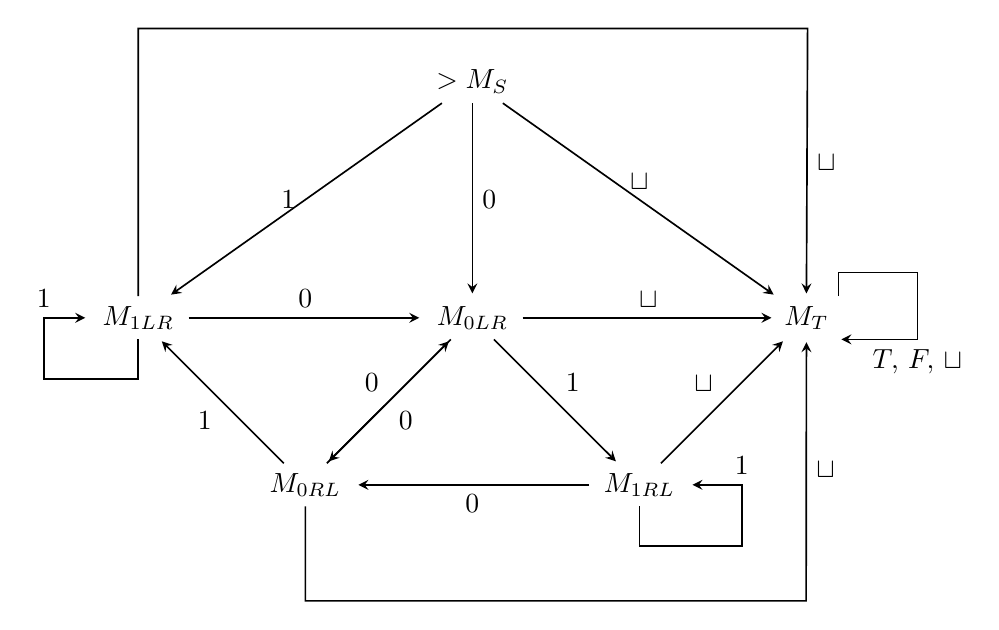
\begin{tikzpicture}[->,>=stealth, shorten >=1pt,semithick,node distance=3.0cm,auto]

		\node(q_1)                  {$\,>M_S\,$};
		\node(q_2) [below of = q_1] {$\,M_{0LR}\,$};
		\node(q_4) [below left of = q_2] {$\,M_{0RL}\,$};
		\node(q_5) [below right of = q_2] {$\,M_{1RL}\,$};
		\node(q_3) [above left of = q_4] {$\,M_{1LR}\,$};
		\node(q_6) [above right of = q_5] {$M_T$};

		\draw[->] (q_1) -- node {$0$} (q_2);
		\draw[->] (q_1) -- node[midway, above] {$\sqcup$} (q_6);
		\draw[->] (q_1) -- node[midway, left] {$1$} (q_3);
		\draw[->] (q_2) -- node {$\sqcup$} (q_6);
		\draw[->] (q_2) -- node {$1$} (q_5);
		\draw[->] (q_2) -- node {$0$} (q_4);
		\draw[->] (q_3) -- node {$0$} (q_2);
		\draw (q_3.south) -- ++(0,-0.5cm) -| ++(-1.2cm,0) |- (q_3.west) node[midway, above] {1};
		\draw (q_3.north) -- ++(0,3.4cm) -| ++(8.5cm,0) -- (q_6.north) node[midway, right] {$\sqcup$};
		\draw[->] (q_5) -- node {$0$} (q_4);
		\draw[->] (q_5) -- node {$\sqcup$} (q_6);
		\draw (q_5.south) -- ++(0,-0.5cm) |- ++(1.3cm,0) |- (q_5.east) node[midway, above] {1};
		\draw[->] (q_4) -- node {$0$} (q_2);
		\draw[->] (q_4) -- node {$1$} (q_3);
		\draw (q_4.south) -- ++(0,-1.2cm) -| ++(6.36cm,0) -- (q_6.south) node[midway, right] {$\sqcup$};
		\draw (q_6.north east) -- ++(0,0.3cm) -| ++(1cm,0) |- (q_6.south east) node[midway, below]
		{$T,\,F,\,\sqcup$};

	\end{tikzpicture}
	\vspace{-0.3cm}
\end{center}
%\clearpage


\begin{tcolorbox}[colback=yellow!15!white, colframe=blue!50!white,
	fonttitle=\bfseries\Large, title = Γραμματική και συντακτικό δένδρο]

\vspace{+0.5cm}
\begin{center}
	\begin{tikzpicture}[->,>=stealth, shorten >=1pt,semithick,node distance=3.0cm,auto]

		\node(q_1)                  {$\overset{\lor}{R}$};
		\node(q_2) [below of = q_1] {$T\,R_\sqcup$};
		\node(q_4) [below left of = q_2] {$\,M_{0RL}\,$};
		\node(q_5) [below right of = q_2] {$\,M_{1RL}\,$};
		\node(q_3) [above left of = q_4] {$\,M_{1LR}\,$};
		\node(q_6) [above right of = q_5] {$L$};
		\node(q_60) [above right of = q_6] {$0$};
		\node(q_61) [below right of = q_6] {$1$};

		\draw[->] (q_1) -- node {$0$} (q_2);
		\draw[->] (q_1) -- node[midway, above] {$\sqcup$} (q_6);
		\draw[->] (q_1) -- node[midway, left] {$1$} (q_3);
		\draw[->] (q_2) -- node {$\sqcup$} (q_6);
		\draw[->] (q_2) -- node {$1$} (q_5);
		\draw[->] (q_2) -- node {$0$} (q_4);
		\draw[->] (q_3) -- node {$0$} (q_2);
		\draw (q_3.south) -- ++(0,-0.5cm) -| ++(-1.2cm,0) |- (q_3.west) node[midway, above] {1};
		\draw (q_3.north) -- ++(0,3.4cm) -| ++(8.5cm,0) -- (q_6.north) node[midway, right] {$\sqcup$};
		\draw[->] (q_5) -- node {$0$} (q_4);
		\draw[->] (q_5) -- node {$\sqcup$} (q_6);
		\draw (q_5.south) -- ++(0,-0.5cm) |- ++(1.3cm,0) |- (q_5.east) node[midway, above] {1};
		\draw[->] (q_4) -- node {$0$} (q_2);
		\draw[->] (q_4) -- node {$1$} (q_3);
		\draw (q_4.south) -- ++(0,-1.2cm) -| ++(6.36cm,0) -- (q_6.south) node[midway, right] {$\sqcup$};
		\draw[->] (q_6) -- node {$F$} (q_60);
		\draw[->] (q_6) -- node[left] {$T$} (q_61);
		\draw (q_6) -- ++(1.25cm,0.75cm) -- ++(0.75cm,0) -- ++(0,-0.7cm) -- ++(-1.65cm,0) node[midway, above]
		{$\sqcup$}
		(q_6);
		{$\sqcup$};
		\draw[->] (q_60) -- ++(0.5cm,0) -- ++(0,-2.3cm) -- ++(-2.53cm,0) node {} (q_6);
		\draw[->] (q_61) -- ++(0.5cm,0) -- ++(0,1.95cm) -- ++(-2.53cm,0) node {} (q_6);

	\end{tikzpicture}
	\vspace{+0.6cm}
\end{center}


\end{tcolorbox}


\begin{center}
	%\vspace{2em}
	\noindent\rule{\linewidth}{0.5pt}
	%\vspace{2em}
\end{center}
\clearpage